\documentclass[twocolumn]{IEEEtran}
\usepackage{epsfig}
%-----------------------

\begin{document}


\title{Incremental Improvements of Software Implemented RSA on multiple processors}


\author{Christian Dancke Tuen \& Kine Johnsrud
\thanks{Authors are with the
Department of Computer Science,
University of California, Santa Barbara, CA 93106.
E-mail: \texttt{\{christiandt,kinej\}@umail.ucsb.edu}}
}

%\markboth{IEEE Transactions On Computers, Vol. 51, No. 5, May 2002}
%{Me and You}

\maketitle

\begin{abstract}
RSA is one of the first practicable public-key cryptosystems, and is widely used for secure data transmission. In this paper we present three different algorithms for calculating the modular exponentiation, and measure their impact on overall speed performance of RSA on different types of processors.
\end{abstract}

\section{Introduction}
RSA is an asymmetric key scheme where the encryption key is public, and the decryption key is kept private. The security of RSA is based on the difficulty of factoring the product of two large prime numbers. RSA uses the same computation for both encryption and decryption.

\bigskip

\centerline{$C = M^e \pmod{n}$}
\centerline{$M = C^d \pmod{n}$}

\bigskip

where $n = pq$, and $p$ and $q$ are two large primes. For more information about the mathematics of RSA, refer to Rivest et al.~\cite{rsa}. RSA can be used to encrypt and exchange private messages, as long as the message is smaller than the size of the key. RSA is more often used as a way to sign and verify digital documents. 

In this paper, we will discuss three ways to implement RSA modular exponentiation. We will implement three fast and viable methods, called the binary method, recoding binary method, and montgomery exponentiation method. We have chosen to run the algorithms on three different processor architectures, to show the importance of efficiency when the hardware speeds are lower. The three processors are an Intel i7 in a Macbook Air, the main Freescale processor of the UDOO development board, and the Atmel processor of the UDOO development board.

\section{Description}
In this section we will discuss the various algorithms we chose to implement, and their main improvement features. We have implemented the binary method, recoding binary method, and montgomery exponentiation.

\subsection*{Binary Method}
In the binary method, we represent the exponents $e$ and $d$ in binary, and scan them from left to right. We call the number of bits $k$. For each bit, we perform a squaring, and if the bit is a 1, we also perform a subsequent multiplication. This gives an order of magnitude fewer operations than the naive method, as the maximum number of multiplications is $2(k-1)$.

\subsection*{Recoding Binary Method}
If the binary representation of the exponent contains a lot of 1's, the standard binary method's performance will be worst-case. The recoding method is used to collapse a block of 1's to obtain a sparse representation of the exponent. We need to introduce the $\bar{1}$, to represent -1. An example: $011110 \rightarrow 1000\bar{1}0$. A tradeoff is that this algorithm requires the inverse of $M$ modulo $n$, which is a costly operation and makes these kind of techniques less valuable for RSA.

\subsection*{Montgomery Exponentiation Method}
The Montgomery Exponentiation method is a concept that also uses the Montgomery Product algorithm. This algorithm is best explained by Koc et al.~\cite{koc}, but the idea is that this is a reduction algorithm that performs multiplication faster than the conventional way by using division by powers of 2 (binary shifts), instead of division by n. This algorithm is proven faster than the ones we have previously discussed, but the amount of overhead (pre-calculations) needed makes the effect of the efficient core algorithm hard to detect on our small-numbered set of values.

\begin{table*}[!htb] 
\textbf{Table 1:} Time in milliseconds of 1000 encryptions and decryptions in RSA \\[1em]
    \centering
    \begin{tabular}{|l|l|l|l|}
    \hline
    {\bf Processor}                                 & {\bf Binary}   & {\bf Recoding Binary} & {\bf Montgomery} \\ \hline
    Intel i7 Dual Core 2.0GHz                 & 0.592 & 1.119        & 2.410   \\ \hline
    Freescale i.MX 6 Cortex-A9 Dual Core 1GHz & 5.600 & 8.667        & N/A       \\ \hline
    Atmel SAM3X8E ARM Cortex-M3 CPU           & 12.333 & 36.667        & N/A       \\ \hline
    \end{tabular}
\end{table*}

\section{Setup}
We decided early on in the project not to use any big-number libraries. As we use an Arduino-compatible microcontroller for the low-end processor, we needed to have a comparable library for all the platforms to make the results of the three processors comparable. After doing a lot of research on this, we did not find any libraries that were sufficiently compatible with the microcontroller. In addition to the added benefit of not being bound to the limitations of the library, and not wanting the results to be influenced by the library's own implementation, we decided not to use any big number libraries on any of the processors during testing.

By not using any libraries to handle big numbers, we are restricted to the maximum number size allowed by the processor. As we are comparing the performance across three different processors, we need to use the same values across all, and are thus restricted by the processor with the lowest maximum number size. In this case we are restricted to maximum values of 32 bit during program execution.

All code is implemented using the C programming language.  We wanted to use a "lower-level" programming language than for example Python, so that it would not influence the performance of the implemented algorithms in any major way. As we are using an Arduino-compatible microcontroller for the low-end processor, using C allows us to port the code over to the microcontroller with only slight modifications.

As earlier stated, performance-testing is performed using three different processors. One high-end Intel processor, a middle-performing ARM processor, and a low-end microcontroller. Testing of the Intel processor is done on a 2013 Apple MacBook Air using the OSX operating system. This is a dual-core 2.0GHz, 64 bit processor, and represents the high-end in our testing. The middle-end processor is a Freescale i.MX 6 Cortex-A9 Dual Core 1GHz and is tested using the Ubuntu Linux distribution on a UDOO computer. Finally, the low-end processor is a Atmel SAM3X8E ARM Cortex-M3 CPU also on the UDOO board. This processor was run separately from the rest of the board, and thus communication needed to be handled by using a serial connection. To ensure that the serial communication did not influence the results, no serial communication was made before all test had finished running.

\begin{figure}[!htb] 
\begin{center} 
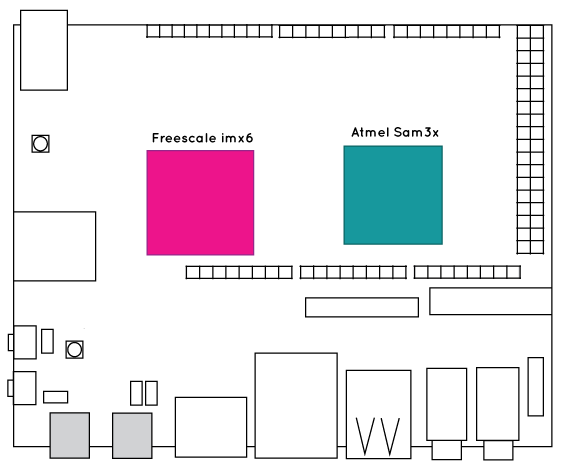
\includegraphics[width=3in]{UDOO_processors.png} 
\caption{Image depicting the two different processors on the UDOO development board} 
\label{fig:proc} 
\end{center} 
\end{figure}

\section{Results}
This section shows the numerical results after running the three different RSA algorithms on three different processor architectures. A set of fixed values are used for p, q, M and e, and all the results are averaged over three measurements. Due to the low number values, all algorithms run both encryption and decryption 1000 times each to get a more accurate number. The montgomery algorithm is not run on the UDOO and the arduino, as the 32-bit limitation would require the numbers to be half the bit-size of the values used for the rest of the measurements. All numbers in the result are per 1000 encryptions and decryptions.

From Table~1 we can see that the binary method performs between 33 \% and 63 \% better than the recoding binary method. The numbers presented here includes calculation of $M$ mod $n$ in each run of the algorithm.

Another noticeable result, is that on the i7 processor, the binary method is approximately 4 times faster than the montgomery method, and the recoding binary method is approximately 2 times faster. As this is not consistent with previous research we will discuss these resuts in the next section.

\section{Discussion}
The difference between the binary method and the recoding binary method can be explained by the nature of the algorithm. Unless the exponents contains large blocks of 1's, the use of recoding will be of little value, and the overhead needed to calculate the inverse modulo will hurt the performance. We did not fabricate a number with a significant amount of subsequent ones, and chose the numbers at random. The numbers used during testing did not have any significant length blocks of ones. With no significantly long blocks, and in addition using relatively small numbers, the performance increase of using recoding binary is drastically reduced compared to the overhead of calculating $M$ mod $n$. As we wanted to show the calculation overhead associated with calculating $M$ mod $n$ in recoding biary, we chose to include this calculation in each run-through of the algorithm. In a real world application, this number would not be calculated each time the encryption/decryption algorithm is run, and therefore does not give the full picture of recoding binary's performance. But omitting the calculation overhead would also not show the algorithms real performance.

As mentioned in the results section, our numbers show that the montgomery method is the slowest of the implemented algorithms even though it is previously proven faster. The strength of the montgomery method is using division by powers of 2 (binary shifts), instead of division by n. These montgomery product operations results in the inner-loop of the montgomery exponentiation function performing well. The downside to this method is that it requires preprocessing as it use $n'$ calculated using the Extended Euclidian Algorithm, and the n-residues. With the small, conceptual numbers used in this experiment, the amount of overhead needed to calculate the n-residues and $n'$ overshadows the effects of faster exponentiation. 

We assume that the performance difference between the montgomery method and binary method will change with increasing number size, changing the best-performing method to the montgomery method, as previously established by the community. If we were to implement support for higher number, we would either have to develop a working big-number library for the Freescale microcontroller, or change to hardware that would support an established big-number library. At the moment, implementing a library for the Freescale seems like the most likely option, but the time required to do this is not feasible within the time allotted to the project.

\section{Conclusion}
The results of our testing did not match the results of mathematical simulation with a 2048-bit key, but the main purpose of this project was to learn RSA on a deeper level, and to understand how such algorithms are implemented in software to make them sufficiently fast. We have managed to implement three versions of the RSA modular exponentiation in C on three different processor platforms, and have discussed how and why our results does not match previously established performance metrics of the comparative speed of the three algorithms.

\bibliographystyle{IEEEbib}
\bibliography{my}


\end{document}